\chapter{Hill Climbing}
\section{Introduction}
In this chapter we focus on the performance of the Hill Climbing search algorithm. Hill Climbing is a non-population based method starting from a single initial solution. This feature coupled with the fact that we are using fine-grained operators makes the starting point in the search space very important. We look initially at the strategy options and examine the parameters used to configure the Hill Climbing algorithm. The results section shows the performance of the algorithm and examines the consequences of different strategy choices for the algorithm in terms of efficiency and success. Initial genome length, zero improvement acceptance, wrapping and the contribution of different operator probabilities are all examined. 



\section{Search Strategy Options}
As in the case of Random Search we fix each trial at 25000 evaluations of the objective function. The operators chosen for Hill Climbing have been designed to allow fine-grained exploration of the search space. Force-up, force-down, shrink and grow (see Section~\ref{operators_hcsa} for a more detailed explanation) operate on a single codon at each iteration, allowing close control of the evolving solution. The four operators are assigned equal probability of occurrence. 



\section{Experimental Conditions}
Table~\ref{hc_param_table} shows the parameters used to configure Hill Climbing. Initial genome length is set at 100 for each of Symbolic Integration, Santa Fe Trail and Blocks, while the more difficult problem of Symbolic Regression is permitted an initial genome length of 200. \emph{Zero improvement acceptance}, which is the strategy of accepting solutions whose score is the same as the current score, it is set to off (i.e. do not accept) for the initial trials. 



\begin{table}[h]
\begin{center}
\begin{tabular}{|l|l|l|l|l|}
\hline
Parameter &\multicolumn{4}{l|}{Problems}\\
\cline{2-1} \cline{3-1} \cline{4-1} \cline{5-1} 
 & Sym Int & Santa Fe & Blocks & Sym Reg  \\
\hline
Number of Trials & 1000 & 1000 & 1000 & 1000 \\
Number of Objective & & & & \\ 
Function Evaluations  & 25000 & 25000 & 25000 & 25000  \\
Initial Genome Length & 100 & 100 & 100 & 200  \\
Initial Genome Length & & & &  \\
Variation Range  & 10\% & 10\% & 10\% & 10\%  \\
Zero Improvement Accept  & off & off & off & off  \\
Probability of Selecting & & & & \\
Shrink Operator  & .25 & .25 & .25 & .25  \\
Probability of Selecting & & & & \\
Grow Operator  & .25 & .25 & .25 & .25  \\
Probability of Selecting & & & & \\
Force-up Operator  & .25 & .25 & .25 & .25 \\
Probability of Selecting & & & & \\
Force-down Operator  & .25 & .25 & .25 & .25  \\
\hline
\end{tabular}
\caption{\label{hc_param_table} Parameters used to configure the Hill Climbing Search Algorithm.}
\end{center}
\end{table}




\section{Results}
The summary results provided in Table~\ref{hc_results_table} show Blocks and Santa Fe Trail as the problems with the highest success rate at 17\% and 15\% respectively. Symbolic Integration has limited success at only 8\% while Symbolic Regression cannot be solved by the algorithm. These figures are significantly lower than the scores recorded by Random Search in the previous chapter, where Symbolic Integration scored 40\%, Santa Fe scored 30\% and Blocks scored 24\%. In an effort to try and understand this difference and improve the performance of Hill Climbing a number of strategy options are analysed in the following sections.


\begin{table}[h]
\begin{center}
\begin{tabular}{|l|l|}
\hline
Problem & Successful Runs \\
\hline
Symbolic Integration & 8\% \\
Santa Fe Trail & 15\% \\
Blocks & 17\% \\
Symbolic Regression & 0\% \\
Spirals & 0\% \\
\hline
\end{tabular}
\caption{ \label{hc_results_table} Results from the Hill Climbing Trials.}
\end{center}
\end{table}


\subsection{Impact of Zero Improvement acceptance}

\emph{Zero improvement acceptance}, the strategy of accepting solutions whose score is the same as the score of the current best performing genome could have provided a means of more extensive exploration of the search space, particularly given the potential for neutral mutation in GE, however permitting acceptance of zero-improvement solutions has no statistically significant impact on success as shown in row three of Table~\ref{zia_table}.   

\begin{table}[h]
\begin{center}
\begin{tabular}{|l|l|l|l|l|}
\hline
Parameter &\multicolumn{4}{l|}{Problems}\\
\cline{2-1} \cline{3-1} \cline{4-1} \cline{5-1} 
 & Sym Int & Santa Fe & Blocks & Sym Reg \\
\hline
Accept Zero Improvement & & & & \\
Solutions & 8\% & 17\% & 11\% & n/a \\
Reject Zero Improvement & & & &  \\
Solutions  & 8\% & 15\% & 17\% & n/a  \\
\hline
Difference & 0\% & +2\% & -6\% & n/a  \\
\hline
\end{tabular}
\caption{\label{zia_table}Impact of Zero Improvement Acceptance on the Hill Climbing Search Algorithm.}
\end{center}
\end{table}


\subsection{Impact of Initial Genome Length}
One of the motivating factors behind the selection of the force-up, force-down, shrink and grow operators was the provision of a mechanism that would allow Hill Climbing create solutions through fine controlled adjustment of the codons within a genome. In this respect it is useful to look at the impact of initial genome length on performance.
 
One of the assumptions with Hill Climbing was that a smaller genome length would suit the algorithm allowing it grow the solution using the fine-grained operators. This would for to be a more efficient use of the given allocation of objective function evaluations rather than starting with a long genome that failed to map and then attempting to shape it, as the initial expression did.

Table~\ref{hc_gl_table} shows the impact of initial genome length on the Symbolic Integration problem when Hill Climbing is employed. Initial genome lengths of 5, 8, 10, 12, 14, 16 and 18 were chosen. Analysis of the results indicate that success rate is independent of initial genome size for this problem. 

\begin{table}[h]
\begin{center}
\begin{tabular}{|l|l|}
\hline
Initial Genome Length & Successful Runs \\
\hline
5 & 8.4\% \\
8 & 8.1\% \\
10 & 8.2\% \\
12 & 9.4\% \\
14 & 6.9\% \\
16 & 6.0\% \\
18 & 7.6\% \\
\hline
\end{tabular}
\caption{\label{hc_gl_table} Effect of Variation of Initial Genome Length on Success Rate for Hill Climbing on the Symbolic Integration Problem.}
\end{center}
\end{table}

 An analysis of these results show that the insignificance of initial genome length is a consequence of the large number of iterations required for Hill Climbing to find a solution. Typically Hill Climbing solutions will have undergone significant variations in size by the time a solution is found.  
This is evidenced by the plot of genome length and fitness for a successful trial shown in Figure~\ref{hc_length}, where the genome is shown to expand and contract as the algorithm moves through the search space. Even with a short starting genome there is always ample time for the solution to shrink and grow through successive iterations. Another feature of this profile is a noticeable decrease in the length of genomes in later iterations.


\subsection{Influence of Operators on Success}
\label{duplicate_solutions}The performance of Hill Climbing is poor relative to that of Random Search in the last chapter. In an effort to understand some of the reasons for this an analysis of the contribution of the operators was undertaken. 

On approach to looking at the contribution of operators is to examine the efficiency of the algorithm as it moves through the search space. Does it, for example, efficiently explore the space? Or, does it spend time re-visiting the same solutions? A measure of this is the degree of duplication of solutions in any given trial.\footnote{The issue of re-visiting previously evaluated solutions is specifically managed in Tabu Search by a mechanism called the Tabu List. The Tabu List is a list of recently visited solutions. The search algorithm is prevented from visiting solutions on the Tabu List.~\cite{tabu}}Table~\ref{hc_symint_altmut_table} shows a figure of 8.4\% duplication in the initial trials on the Symbolic Integration problem. An analysis of specific search trajectories show that the main cause of this duplication is successive occurrences of the shrink and grow operators where a genome first grows in one direction before shrinking back on itself.
This is also graphically illustrated in Figure~\ref{hc_length} which shows the oscillating nature of the search. 


\begin{figure}[]
\centerline{\hbox{
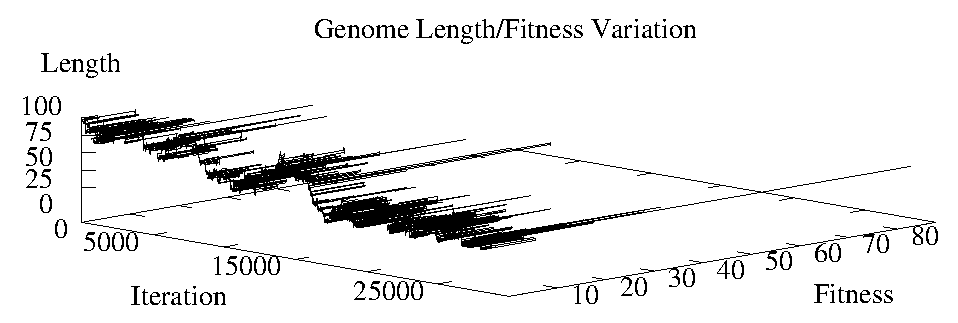
\psfig{file=Chapter6/graphs/length_fitness_variation.ps,width=5in}}}
\caption{\label{hc_length} Variation in Genome Length for a Successful Hill Climbing Trial on the Santa Fe Trail problem.}
\end{figure}

Reducing the probability of the shrink operator should have the effect of reducing duplication with a possible increase in success rates. Table ~\ref{hc_symint_altmut_table} illustrates this in the case of Symbolic Integration where the success rate climbs from 8\% to 14\% when the probability of the shrink operator is reduced to .05 (5\%). We also see the number of duplicate  solutions fall from 8.4\% to 1.6\% under the influence of this change. Tables~\ref{hc_santafe_altmut_table} and ~\ref{hc_blocks_altmut_table} show a similar situation for the Santa Fe and Blocks problems. The Symbolic Regression problem remained unsolved when operator probabilities were modified so a results summary for this problem has not been included.
  
Interestingly while this reduction in the probability of the shrink operator sees similar reduction in duplication for the Santa Fe and Blocks problem we do not see any significant change in the success rate. 
To further underline the fact that reduced duplication in itself does not guarantee higher success rates we can look at the consequences of introducing a coarser operator into the Hill Climbing algorithm.
The introduction of \emph{multiple mutation}, which permits the changing of up to 10\% of a genome's codons in a single iteration, sees the amount of duplicate solutions rise to 13\% while the success rate also rises to 18\% for the Symbolic Integration problem. One has to be cautious here however as the introduction of such a disruptive operator moves the algorithm closer to random search rather than the controlled exploration of the search space envisaged for Hill Climbing. 

\begin{table}[h]
\begin{center}
\begin{tabular}{|l|l|l|}
\hline
Operators                     & Successful             & Percentage    \\
                              & Runs                   & Duplication    \\  
\hline
shrink and grow at .25       & 8\%                     &       8.4\%  \\
shrink and grow at .5        & 14\% (+6\%)             & 1.6\% (-6.8\%) \\
multiple mutation 10\%       & 18\% (+10\%)            & 13\% (+4.6\%) \\
\hline
\end{tabular}
\caption{\label{hc_symint_altmut_table} Effect of variation of operators on success rate for Hill Climbing on the Symbolic Integration problem.}
\end{center}
\end{table}


\begin{table}[h]
\begin{center}
\begin{tabular}{|l|l|l|}
\hline
Operators                     & Successful      & Percentage  \\
                              & Runs            & Duplication \\
\hline
shrink and grow at .25       & 15\%              & 8\%\\
shrink and grow at .05       & 11\% (-4\%)       & 2\% (-6\%)\\
multiple mutation 10\%       & 18\% (+3\%)       & 13\% (+5\%) \\
\hline
\end{tabular}
\caption{\label{hc_santafe_altmut_table} Effect of variation of operators on success rate for Hill Climbing on the Santa Fe Trail problem.}
\end{center}
\end{table}




\begin{table}[h]
\begin{center}
\begin{tabular}{|l|l|l|}
\hline
Operator Probabilities  & Successful Runs & Percentage Duplication \\
\hline
shrink and grow at .25  & 17\%             & 9.3\%\\
shrink and grow at .05  & 16\% (-1\%)      & 3.5\% (-5.8\%)\\
multiple mutation 10\%  & 10\% (-7\%)      & 14\% (+4.7\%) \\
\hline
\end{tabular}
\caption{\label{hc_blocks_altmut_table} Effect of reduced probability for shrink and grow operators on success rate for Hill Climbing on the Blocks problem.}
\end{center}
\end{table}




\section{Characteristics of Solutions found by Hill Climbing}

\begin{table}[h]
\begin{center}
\begin{tabular}{|l|l|l|l|l|}
\hline
Feature & Sym Int & Santa Fe & Blocks & Sym Reg  \\
\hline
Avg Number of Codons & & & &  \\ 
in Solution & 52 & 42 & 50 & n/a  \\
Avg Number of expressed & & & &  \\
Codons in Solution & 15 & 47 & 77  & n/a  \\
Percentage of Solutions & & & & \\
featuring Wrapping & 0\% & 80\% & 70\% & n/a  \\
\hline
\end{tabular}
\caption{\label{hc_results_analysis_table} Analysis of Characteristics from Solutions found by Hill Climbing.}
\end{center}
\end{table}

An examination of the data presented in Table~\ref{hc_results_analysis_table} shows a  high percentage of solutions for Santa Fe (80\%) and Blocks (70\%) that use wrapping. Despite starting with an initial genome length of 100 (+/- 10\%) the Hill Climbing algorithm on these problems consistently moves towards genomes with smaller numbers of codons. In the case of Hill Climbing this move is facilitated by the \emph{shrink} operator. Even when the contribution of this operator is reduced from 25\% to 5\% on the Santa Fe Trail problem the high incidence of wrapping is maintained at 46\% of solutions with the average number of codons rising to 58.

If the ability to migrate to short genomes is eliminated by removing the \emph{shrink} operator altogether the success rate of Hill Climbing on the Santa Fe Trail problem fall significantly from 15\% to 7\%.   
In the case of Symbolic Integration wrapping is not involved in any of the solutions, with the average number of expressed codons (15) less than  half the size of the average number of codons in a solution (52).  Removing the \emph{shrink} operator in this instance sees no change in the success rate. This should be expected given the absence of wrapping found in the original trials.

A curious aspect of these results is the tendency toward shorter  genome lengths when GE could just as easily ignore the unexpressed codons to the right. An examination of the search trajectory however reveals situations in which  we typically see large numbers of iterations between changes in the score, during this period the genome shrinks and grows repeatedly under the influence of the shrink and grow operators. It is during this period when the genome is shortest that we are more likely to change a codon that results in an improved score.

In the case of Blocks, which have the highest percentage of wrapping, the number of expressed codons is far greater than the average number of codons found in a solution. An analysis of the results shows that solutions often use multiple wrap events. Some of the underlying causes of this will be explored in later chapters.

\subsection{Analysis of search trajectory}
A clear indication of the difficulty faced by Hill Climbing on these problems is provided by an analysis of the search trajectories of successful Hill Climbing trials. A representative plot is shown in Figure~\ref{hc_search1}.

This  plot of the search trajectory shows the Hill Climbing algorithm negotiating its way through low scoring solutions before making a quantum leap to the optimum solutions. 

\begin{figure}[]
\centerline{\hbox{
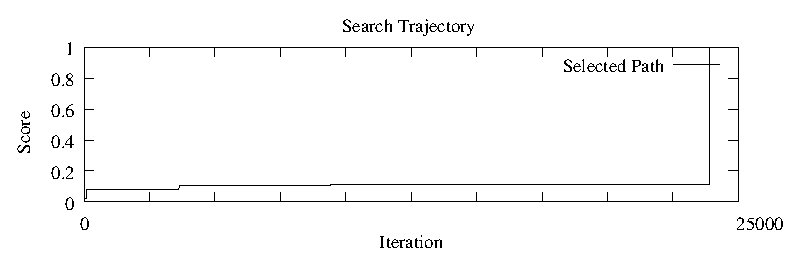
\psfig{file=Chapter6/graphs/search_trajectory_1.ps,width=5in}}}
\caption[Search Trajectory for a successful Hill Climbing trial]{Search Trajectory for a successful Hill Climbing trial on the Santa Fe Trail Problem}
\label{hc_search1}
\end{figure}



\section{Problem Difficulty}
The results for Hill Climbing also challenge some of the assumptions we made about problem difficulty in the previous chapter, where the results from Random Search suggested that Symbolic Integration was the easiest of the problems to solve. Hill Climbing scored 8\% on this problems against a score of 40\% for Random Search, indicating that the difficulty of a problem is relative to the search method being used. Again, this is supported by the results from the Santa Fe trail and Blocks problems where Hill Climbing scores 15\% and 17\% respectively while Random Search clearly finds Santa Fe easier (scoring 30\%) than Blocks (scoring 24\%).


\section{Summary}
In this chapter we have looked at the performance of Hill Climbing a local search Metaheuristic. The impact of accepting or rejecting \emph{zero improvement} solutions was examined and found to have no significant effect. We also looked at the influence of the length of the initial Genome on success rates and examined the contribution of the selected operators in terms of efficiency and effectiveness. 
We looked at the tendency toward short genomes lengths and the use of wrapping to find solutions. This was particularly evident in the case of Santa Fe Trail and Blocks.

Overall the performance of Hill Climbing has been poor relative to the efforts of Random Search in the previous chapter. Even when it does succeed we see a quantum leap from very low fitness to maximum fitness rather than a gradual ascent through intermediate levels of fitness. While many of the attempts to modify the strategy options associated with Hill Climbing saw no significant improvement in the success rate, the introduction of a more disruptive mutation operator did see a significant increase in the score. Finally, we have re-assesed some of our assumptions about problem difficulty based on the comparative results of Hill Climbing and Random Search.





















































